\documentclass[12pt, a4paper]{article}

% --- Paquetes básicos ---
\usepackage[utf8]{inputenc}
\usepackage[spanish]{babel}
\usepackage[margin=2.5cm]{geometry}
\usepackage{graphicx}
\usepackage{amsmath, amssymb}
\usepackage{fancyhdr}

% --- Configuración del Título ---
\title{Bloque 2: Simulación de Carga de Trabajo y Monitorización}
\author{Juan Reche Aguilar}
\date{\today}

% --- Configuración de Encabezados ---
\pagestyle{fancy}
\fancyhf{}
\rhead{Ingeniería de Servidores}
\lhead{Juan Reche Aguilar}
\cfoot{\thepage}

\begin{document}

\maketitle

\tableofcontents
\newpage

\section{Ejercicio. Ejecutar "Hello World"}

\begin{figure}[htbp]
    \centering

    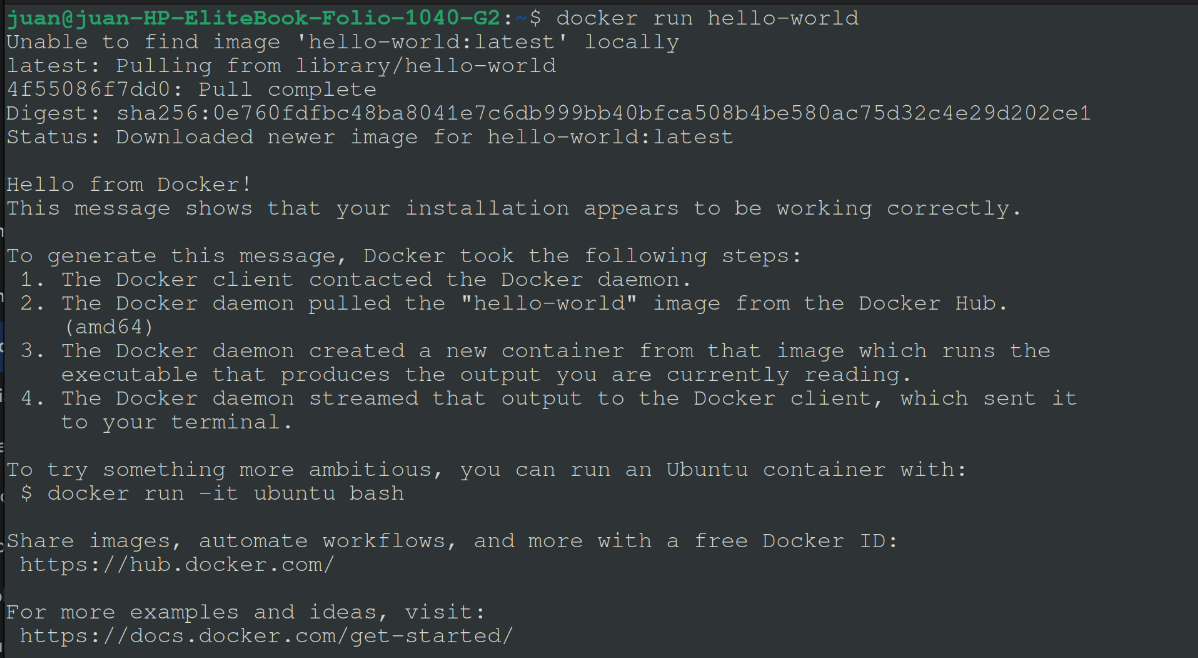
\includegraphics[width=1\textwidth]{../../capturas1/ejercicio1.png}

    %\caption{Descripción del gráfico o figura del ejercicio.}

    \label{fig:mi_grafico}
\end{figure}

Como se puede observar en la Captura \ref{fig:mi_grafico}, se ejecuta el conenedor de Docker con el comando 
\texttt{docker run hello-world} sin el uso de root. 

\end{document}